\section{Leistungshalbleiter in der Leistungselektronik}

\subsection{Rolle der Leistungshalbleiter im Energiesystem}

Leistungshalbleiter dienen der verlustarmen, schnellen und steuerbaren Umsetzung elektrischer Energie.
Sie arbeiten im Gegensatz zu linearen Bauelementen ausschliesslich in den Zuständen:
\begin{itemize}
\item \textbf{leitend} (niedriger Spannungsabfall),
\item \textbf{sperrend} (hohe Sperrspannung),
\item \textbf{umschaltend} (Übergangszustand).
\end{itemize}

Damit realisieren sie:
\begin{itemize}
\item Gleichrichtung,
\item Phasenanschnitt,
\item Taktbetrieb (PWM),
\item Umrichtung von Spannung, Strom und Frequenz.
\end{itemize}

Grundlegende Kenngrössen:
\[
U_{RRM},\quad I_{F},\quad U_F,\quad t_{on},\ t_{off},\quad P_{cond},\ P_{sw}.
\]

\subsection{Physikalische Grundlagen der Halbleiterbauelemente}

Alle Leistungshalbleiter beruhen auf pn-Übergängen.

Sperrbetrieb:
\[
i \approx 0,\qquad u \le U_{RRM}
\]

Durchlassbetrieb:
\[
i \gg 0,\qquad u \approx U_{on}
\]

Die maximale Sperrspannung wird bestimmt durch:
\begin{itemize}
\item Dicke der Sperrschicht,
\item Dotierung,
\item Feldverteilung im pn-Übergang.
\end{itemize}

Thermische Belastung:
\[
\boxed{T_j = T_{amb} + R_{th} \cdot P_V}
\]
mit:
\begin{itemize}
\item $T_j$: Sperrschichttemperatur,
\item $R_{th}$: thermischer Widerstand,
\item $P_V$: Verlustleistung.
\end{itemize}

\subsection{Diode als Leistungsschalter}

\subsubsection{Betriebszustände}

Die Leistungsdiode besitzt zwei stabile Zustände:

\textbf{Durchlass:}
\[
u_D > 0,\qquad i_D > 0
\]

\textbf{Sperre:}
\[
u_D < 0,\qquad i_D \approx 0
\]

Ideales Modell:
\[
u_D =
\begin{cases}
0, & i_D > 0 \\
\infty, & i_D = 0
\end{cases}
\]

\subsubsection{Statisches Durchlassmodell}

Reales Modell:
\[
\boxed{u_D = U_{D0} + r_D \, i_D}
\]

Verlustleistung:
\[
\boxed{P_D = U_{D0} \, I_{D,\mathrm{avg}} + r_D \, I_{D,\mathrm{RMS}}^2}
\]

Interpretation:
\begin{itemize}
\item $U_{D0}$ dominiert bei kleinen Strömen,
\item $r_D$ dominiert bei grossen Strömen.
\end{itemize}

\begin{center}
    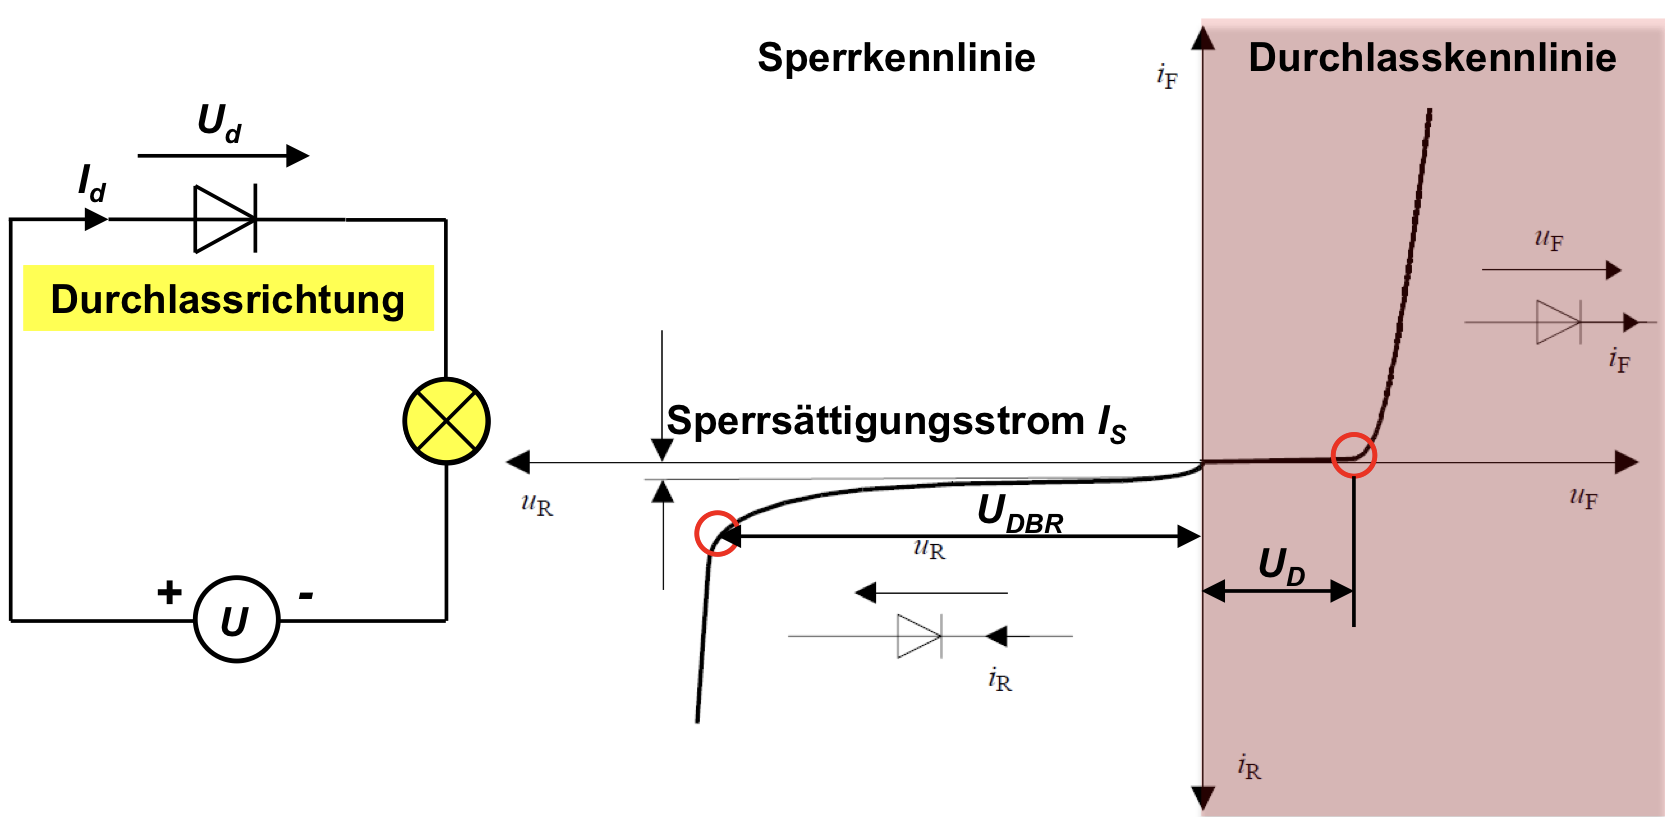
\includegraphics[width=0.85\linewidth]{images/Didodekennlinie.png}
\end{center}
\begin{center}
    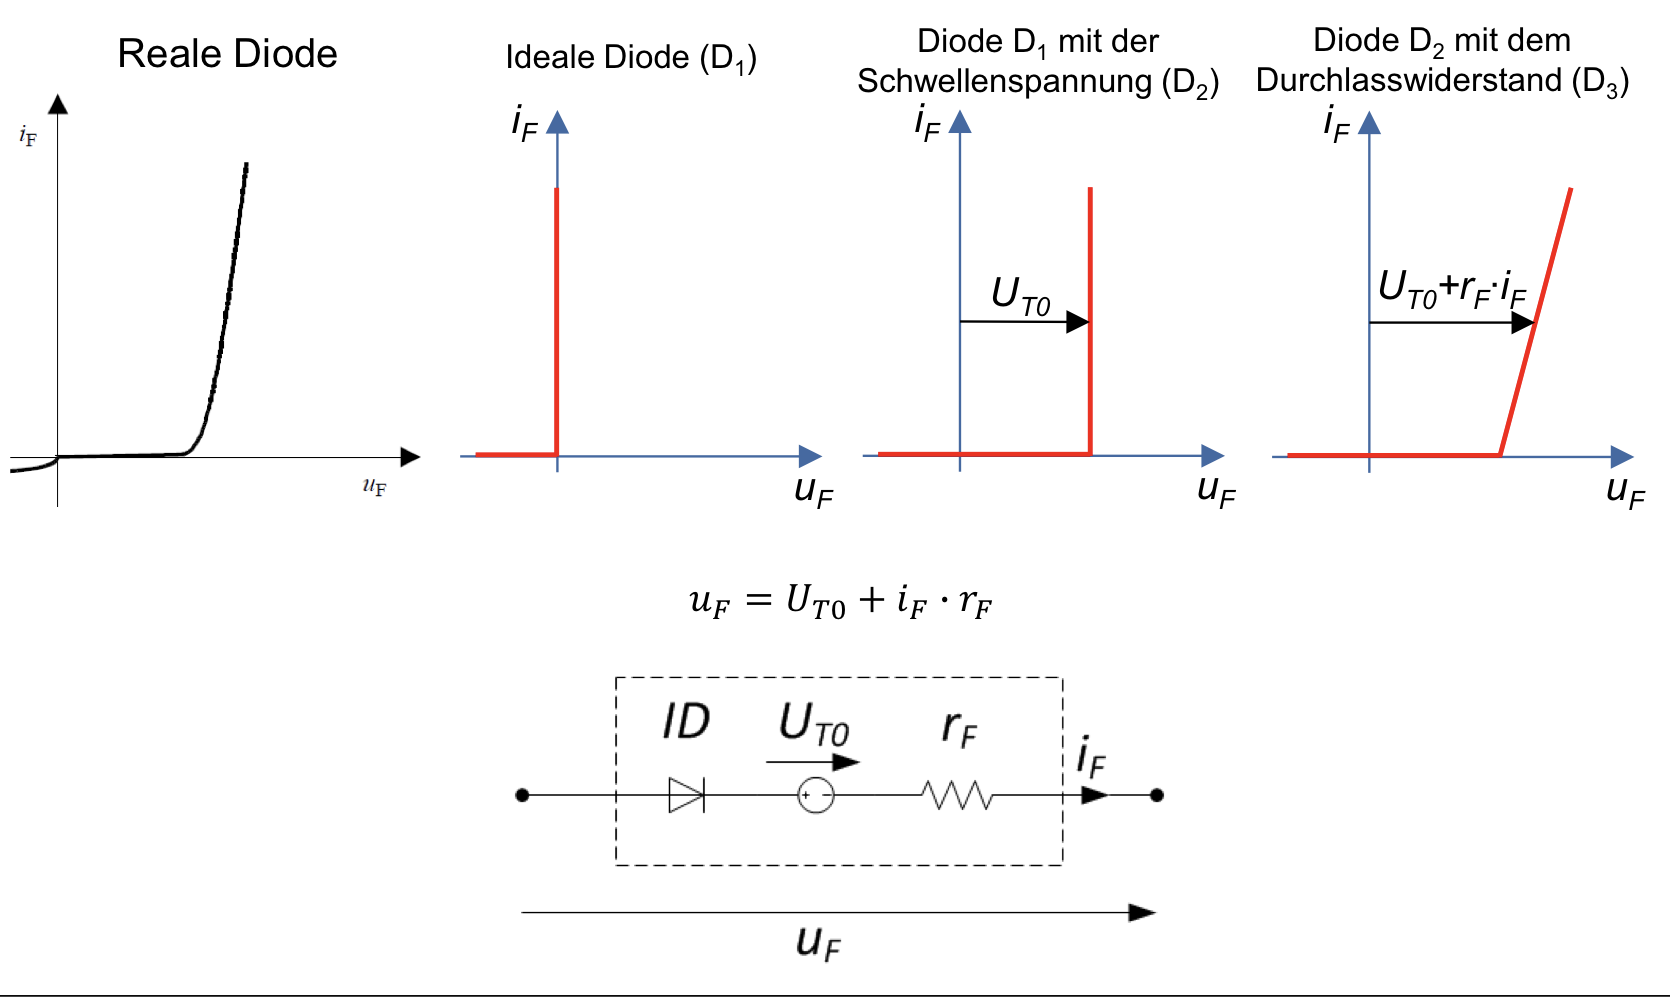
\includegraphics[width=0.85\linewidth]{images/didodeunterschied.png}
\end{center}
\subsubsection{Dynamisches Schaltverhalten}

Beim Übergang von Durchlass nach Sperre wird Ladung aus der Sperrschicht entfernt.

Rückerholstrom:
\[
i_{rr}(t)
\]

Rückerholladung:
\[
\boxed{Q_{rr} = \int_0^{t_{rr}} i_{rr}(t)\,dt}
\]

Zusätzliche Schaltverluste:
\[
\boxed{P_{sw,D} \approx f_s \, U_R \, Q_{rr}}
\]

Physikalische Bedeutung:
\begin{itemize}
\item grosse $Q_{rr}$ $\Rightarrow$ hohe Verluste,
\item schnelle Dioden notwendig für hohe $f_s$.
\end{itemize}

\begin{center}
    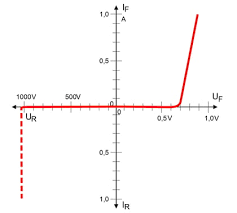
\includegraphics[width=0.85\linewidth]{images/rueckerhol.png}
\end{center}

\subsection{Thyristor (SCR)}

\subsubsection{Vier-Schichten-Struktur und Zündprinzip}

Der Thyristor besitzt eine PNPN-Struktur.

Zündbedingung:
\[
u_{AK} > 0 \quad \text{und} \quad i_G > 0
\]

Nach dem Zünden:
\[
\boxed{\text{Selbsthaltung durch innere Rückkopplung}}
\]

Haltestrom:
\[
\boxed{i_A > I_H}
\]

Abschalten nur durch:
\begin{itemize}
\item Stromnulldurchgang,
\item externe Kommutierung.
\end{itemize}

\begin{center}
    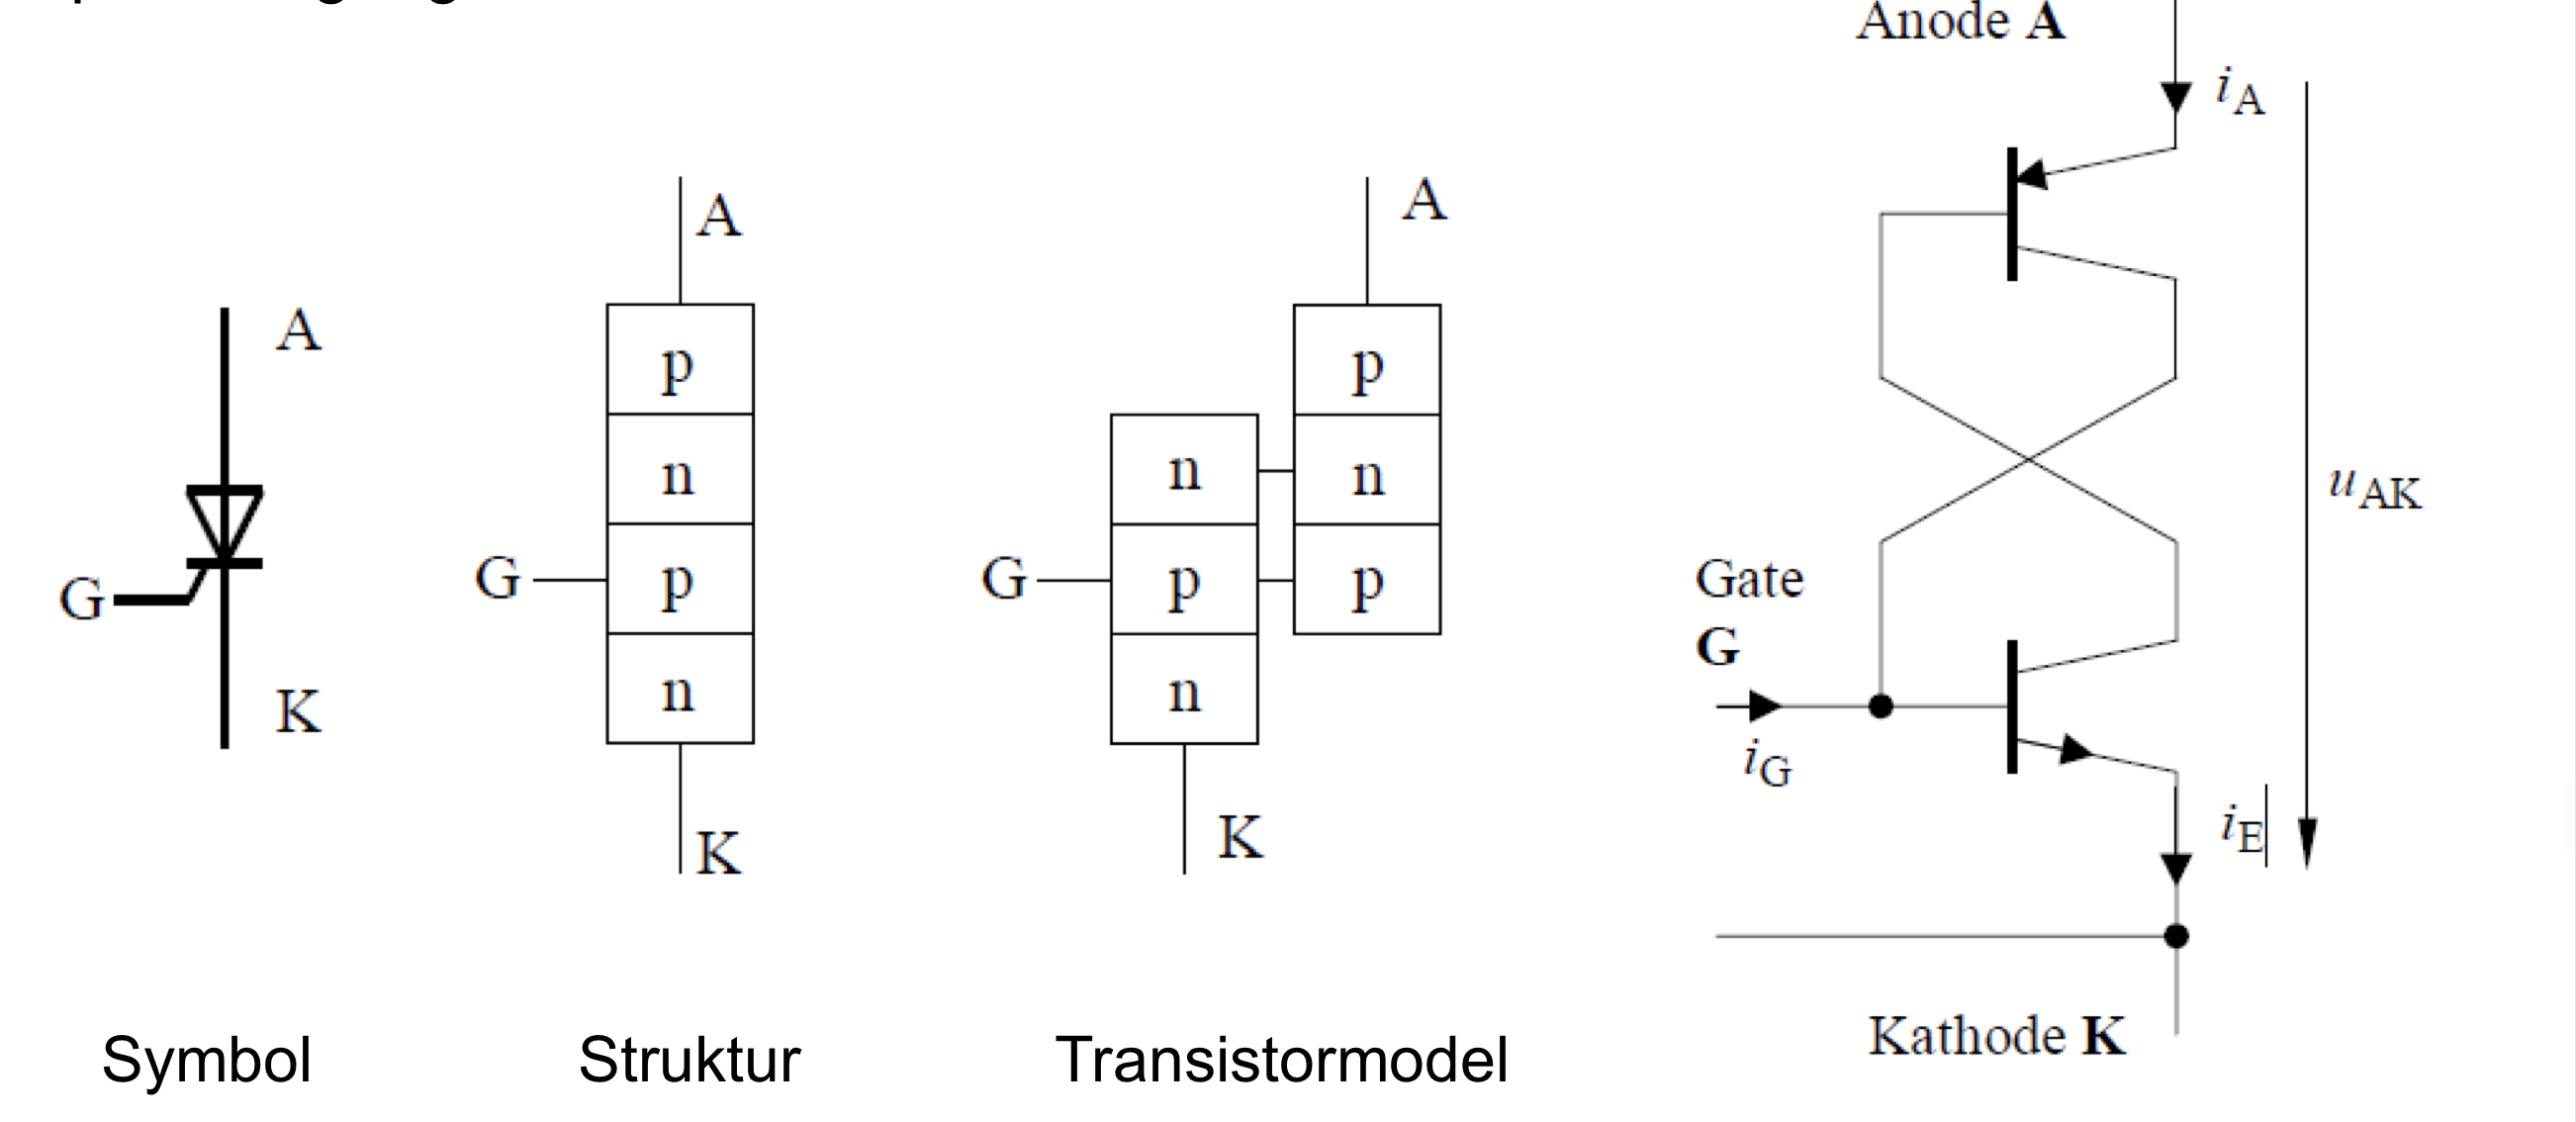
\includegraphics[width=0.85\linewidth]{images/thyristor.png}
\end{center}

\subsubsection{Statisches Modell und Verluste}

\[
\boxed{u_T = U_{T0} + r_T \, i_T}
\]

\[
\boxed{P_T = U_{T0} \, I_{T,\mathrm{avg}} + r_T \, I_{T,\mathrm{RMS}}^2}
\]

Zusätzliche Kenngrössen:
\[
\frac{di}{dt}_{\max},\qquad \frac{du}{dt}_{\max}
\]

Bedeutung:
\begin{itemize}
\item Begrenzen Zündstromanstieg,
\item Schutz durch Snubber notwendig.
\end{itemize}

\subsection{Leistungs-MOSFET}

\subsubsection{Gate-gesteuerter Feldeffekttransistor}

Leitbedingung:
\[
\boxed{u_{GS} > U_{th}}
\]

Im leitenden Zustand:
\[
\boxed{u_{DS} = r_{DS,on} \, i_D}
\]

Charakteristisch:
\begin{itemize}
\item Mehrheitsladungsträger,
\item kein Speicherladungseffekt,
\item sehr schnelles Schalten.
\end{itemize}

\begin{center}
    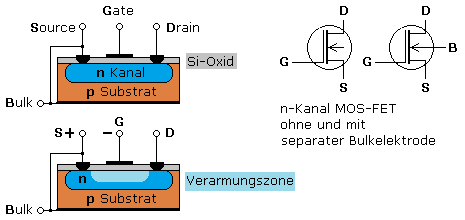
\includegraphics[width=0.85\linewidth]{images/MOSFET.png}
\end{center}

\subsubsection{Dynamisches Modell und Gate-Ladung}

Gate-Ladung:
\[
Q_G = Q_{GS} + Q_{GD}
\]

Schaltzeit:
\[
t_{on} \approx \frac{Q_G}{I_G}
\]

Schaltverluste:
\[
\boxed{P_{sw,M} \approx f_s \int u_{DS}(t)i_D(t)\,dt}
\]

\subsection{IGBT}

\subsubsection{Hybridstruktur MOS–Bipolar}

Der IGBT kombiniert:
\begin{itemize}
\item spannungsgesteuertes MOS-Gate,
\item stromtragende bipolare Struktur.
\end{itemize}

Leitbedingung:
\[
\boxed{u_{GE} > U_{th}}
\]

Durchlassmodell:
\[
\boxed{u_{CE} = U_{CE0} + r_{CE} \, i_C}
\]

\begin{center}
    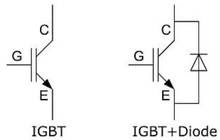
\includegraphics[width=0.85\linewidth]{images/IGBT.png}
\end{center}

\subsubsection{Tail-Strom und Abschaltverluste}

Beim Abschalten verbleibt Speicherladung im Driftgebiet.

Tail-Strom:
\[
i_{tail}(t)
\]

Zusätzliche Verluste:
\[
\boxed{P_{off} \gg P_{on}}
\]

Konsequenz:
\begin{itemize}
\item langsamer als MOSFET,
\item dafür geringere Leitverluste bei grossen Strömen.
\end{itemize}

\subsection{Vergleich der Bauelemente}

\begin{center}
\begin{tabular}{l|c|c|c|c}
 & Diode & Thyristor & MOSFET & IGBT \\
\hline
Steuerbar & nein & Zünden & ja & ja \\
Abschaltbar & ja & nein & ja & ja \\
Schaltfreq. & mittel & tief & sehr hoch & mittel \\
Leitverluste & klein & klein & klein bei klein $I$ & klein bei gross $I$ \\
Speicherladung & ja & ja & nein & ja \\
\end{tabular}
\end{center}
\subsection{Safe Operating Area (SOA)}

Die Safe Operating Area beschreibt den zulässigen Arbeitsbereich eines Leistungshalbleiters
im Strom–Spannungs–Diagramm.

Zulässige Grenzbedingungen:
\[
\boxed{
\begin{aligned}
u &< U_{RRM} \\
i &< I_{\max} \\
P &= u \cdot i < P_{\max} \\
\frac{di}{dt} &< \left(\frac{di}{dt}\right)_{\max} \\
\frac{du}{dt} &< \left(\frac{du}{dt}\right)_{\max}
\end{aligned}
}
\]

Physikalische Bedeutung:
\begin{itemize}
\item Begrenzung durch Durchbruchspannung,
\item Begrenzung durch thermische Überlast,
\item Begrenzung durch sekundären Durchbruch (bipolare Bauelemente).
\end{itemize}

Die Einhaltung der SOA ist zwingend für den sicheren Betrieb.


\subsection{Zusammenfassung der Verlustmechanismen}

Gesamtverluste:
\[
\boxed{P_V = P_{cond} + P_{sw}}
\]

mit:
\[
P_{cond} = U_0 I_{\mathrm{avg}} + r I_{\mathrm{RMS}}^2
\]
\[
P_{sw} = f_s \int u(t)i(t)\,dt
\]

Thermische Auslegung:
\[
T_j = T_{amb} + R_{th} P_V < T_{j,\max}.
\]
\subsection{Vereinfachte Schaltverlustrechnung}

Bei näherungsweise linearem Spannungs- und Stromverlauf während des Schaltens gilt:

\paragraph{Einschaltverlust}

\[
\boxed{E_{on} \approx \frac{1}{2} U \, I \, t_{on}}
\]

\paragraph{Ausschaltverlust}

\[
\boxed{E_{off} \approx \frac{1}{2} U \, I \, t_{off}}
\]

Mittlere Schaltverluste:

\[
\boxed{
P_{sw} = f_s \left(E_{on} + E_{off}\right)
}
\]

Konsequenzen:
\begin{itemize}
\item $f_s \uparrow \Rightarrow P_{sw} \uparrow$
\item $t_{on}, t_{off}$ klein $\Rightarrow$ geringe Verluste.
\end{itemize}

\subsection{Thermische Widerstandskette}

\[
\boxed{R_{th,tot} = R_{th,jc} + R_{th,ck} + R_{th,ka}}
\]

Temperaturen:

\[
T_j = T_{amb} + R_{th,tot} P_V
\]
\[
T_c = T_j - R_{th,jc} P_V,
\qquad
T_k = T_c - R_{th,ck} P_V
\]

Grenzbedingung:
\[
\boxed{T_j < T_{j,\max}}
\]
\subsection{Vereinfachte Schaltverlustrechnung}

Bei näherungsweise linearem Spannungs- und Stromverlauf während des Schaltens gilt:

\paragraph{Einschaltverlust}

\[
\boxed{E_{on} \approx \frac{1}{2} U \, I \, t_{on}}
\]

\paragraph{Ausschaltverlust}

\[
\boxed{E_{off} \approx \frac{1}{2} U \, I \, t_{off}}
\]

Mittlere Schaltverluste:

\[
\boxed{
P_{sw} = f_s \left(E_{on} + E_{off}\right)
}
\]

Konsequenzen:
\begin{itemize}
\item $f_s \uparrow \Rightarrow P_{sw} \uparrow$
\item $t_{on}, t_{off}$ klein $\Rightarrow$ geringe Verluste.
\end{itemize}
